\documentclass{article}

\usepackage[margin=1in]{geometry}
\usepackage{parskip}
\usepackage{datetime}
\usepackage{url}
\usepackage{hyperref}
\usepackage[utf8]{inputenc}
\usepackage{graphicx}

\newdateformat{required}{\twodigit{\THEMONTH}/\twodigit{\THEDAY}/\THEYEAR}
\raggedbottom
\begin{document}

\begin{titlepage}
    \begin{center}
        \begin{huge}
        House in Your Head \\[1cm]
        Team G1-FrigidWaters \\[2.2cm]
        { \bfseries System Requirements Specification } \\[1cm]
        Cycle \# 2\\[2.2cm]
        Date: \required\today\\[1cm]
        \end{huge}
    \end{center}
    \null \vfill
    \begin{large}
        Team Members: \\[0.5cm]
        Name: Samuel Bever\\[0.5cm]
        Name: Michael Conway\\[0.5cm]
        Name: Joseph Muoio\\[0.5cm]
        Name: Kyle Patron\\[0.5cm]
        Name: Kevin Zakszewski
    \end{large}
\end{titlepage}
\section*{\centering Table of Contents}
\makeatletter
\@starttoc{toc}
\newcommand{\hsubsubsection}{
\@startsection{subsubsection}{3}{\z@}%
                                     {-3.25ex\@plus -1ex \@minus -.2ex}%
                                     {-1.5ex \@plus -.2ex}% Formerly 1.5ex \@plus .2ex
                                     {R\normalfont\normalsize}}
\newcommand{\hparagraph}{
\@startsection{paragraph}{4}{\z@}%
                                     {-3.25ex\@plus -1ex \@minus -.2ex}%
                                     {-1.5ex \@plus -.2ex}% Formerly 1.5ex \@plus .2ex
                                     {R\normalfont\normalsize}}
\newcommand{\hsubparagraph}{
\@startsection{subparagraph}{5}{\z@}%
                                     {-3.25ex\@plus -1ex \@minus -.2ex}%
                                     {-1.5ex \@plus -.2ex}% Formerly 1.5ex \@plus .2ex
                                     {R\normalfont\normalsize}}
\setcounter{secnumdepth}{5}
\makeatother
\newpage
 

\section{Introduction}

\subsection{Purpose}

The purpose of this document is to describe the requirements of the House in
Your Head system. The remaining sections define the scope of the project,
introduce necessary language and definitions, give an overview of the project,
and lay out the requirements for the system.

\subsection{Scope}

% TODO: Describe scope of applications
% Define the scope of the functions that will be developed for
% managing the house appliances in addition to the interfaces of the devices. 

This system is intended as a way for users to make basic state changes in an
Insteon automated home setting using a Brain Computer Interface. Basic states to be
changed are characterized by having a binary setting (on or off). This system
also includes a user interface that is controlled by binary actions. Complex
systems with multiple or intermediate states are out of the scope of the Brain
Computer Interface portion of this project. Some settings that have multiple
states can be maintained by an administrator. This administrator will need to
do so via a mouse and keyboard. 

%TODO talk more about HAS here Kyle
%TODO also talk about what devices we support.

The potential users of this system will be people who suffer from ALS, as well
as the administrators who will be assisting the general users set up the
program and software. Dr. Sara Feldman, The ALS Center of Hope at Drexel
University, and Professor Jeff Salvage are the primary stakeholders and
sponsors of this project.

\subsection{Definitions, Acronyms, and Abbreviations}

\begin{description}
    \item[EEG] Can refer to:
        \begin{itemize}
            \item Electroencephalography - Recording of the brain's electrical
                activity 
	        \item Electroencephalogram - The device that is used to record the
	            brain's electrical activity
        \end{itemize}
    \item[Emotiv] The electroencephalogram hardware device, created by Emotiv
        Limited, used to read the user's brain activity (EEG)
        % TODO cite?
    \item[Brain Computer Interface (BCI)] The class of devices that the Emotiv
        belongs to
    \item[Amyotrophic Lateral Sclerosis (ALS)] A neurodegenerative disorder
        that our target users suffer from. The main characteristics of ALS
        that we are concerned with in the scope of this project are the
        limited movement and mobility to complete paralysis.
    \item[Insteon] The suite of home-automation devices that this system will
        interface with; see \url{http://www.insteon.com/}
\end{description}


\subsection{Overview}

Section 2 discusses the background and context of this system and indicates
general requirements and constraints. Section 3 lists specific requirements
for the system.

\newpage

\section{Overall Description}

\subsection{Product Perspective}

\subsubsection{System Interface}

\begin{figure}[h!]
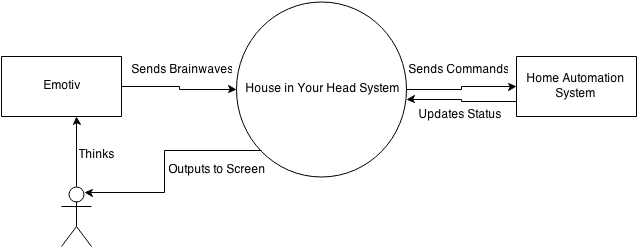
\includegraphics[width=\textwidth]{Senior_Design_Context_Diagram_V1.png}
\caption{Context Diagram of the system}
\label{fig:contextdia}
\end{figure}

The user wears an Emotiv headset which sends information about their thoughts
to the connected computer. From here, the information is interpreted as
commands to be sent to the home automation controller based on the EEG selections for the current GUI screen. The controller in turn sends 
commands to the Insteon system to command the connected components, such as the television and lights.
%TODO Joe Update wording here
%Home Automation system is an external entity.  
%Does it mean your system only transforms the signals from Emotiv to Home Automation System?  

\subsubsection{User Interface}
% TODO Joe and Kevin update wording here
The user interface consists of the Emotiv device and a graphical user
interface to be shown on a standard computer display. The Emotiv device is
attached to the user's head and reads their brain's electrical impulses, which
are generated in response to prompts from the display. These impulses are
then converted into commands that are then used as input. The exact input will
be one of two states – neutral or active. Because there are only two states
for the input, the complexity of the user interface as a whole is
intentionally limited. This will allow for a simpler user experience and
easy usability. The commands sent to the HAS is based on what is shown on screen when the user selects.

\subsubsection{Hardware Interfaces}
%Kyle
The system interfaces with both the Emotiv Epoc device and the Insteon
PowerLinc Modem via Universal Serial Bus (USB).

\subsubsection{Software Interfaces}

The Emotiv framework provides a set of functions which allows access to the
EEG data.

\subsubsection{Communication Interfaces}

The system communicates with components of the Insteon system via its USB
connection to the PowerLinc Modem, using the Insteon-defined command set.

\subsubsection{Memory Constraints}

The system runs on consumer systems, so its RAM footprint must be limited
accordingly.

\subsubsection{Operations}
% Kyle
The system has two modes of operation, calibration and active. Calibration
consists of having the Patient (as described in section \ref{sec:UserChar})
train the system to associate certain brainwaves with actions.

Active mode occurs after calibration has finished, and is the general
operations described in this document.

\subsubsection{Site Adaption Requirements}
The system must run in both a home and a healthcare setup, as long as an
Insteon system consisting of supported home control devices is present. No
modifications to the system, other than configuration for available devices,
are required to change between these two environments.

However, it is expected that not all types of Insteon devices will be
supported in the initial release, and more will be developed over time. It
must be possible for a competent developer to add support for a new device
without undue modification to the rest of the system.

\subsection{Product Functions}

\begin{itemize}
\item Gather EEG data from the user
\item Analyse and filter the EEG data to make a reliable signal
\item Provide user with a menu from which to select home automation actions
\item Perform selected home automation actions
\end{itemize}

\subsection{User Characteristics}
\label{sec:UserChar}
Two categories of users are considered:

\begin{description}
    \item[Patients] are those suffering from ALS who are the primary users of
        the system. The severity of the disorder in each patient can range
        from limited mobility to full paralysis; the system assumes the
        latter.
    \item[Caretakers] are individuals not suffering from ALS who are
        responsible for Patients. They are assumed to be present during system
        setup and administrative tasks, but \textbf{not} during other use
        cases.
    \item[Device Support Developers] are those who wish to add support for an
        unsupported Insteon device, or a custom device that conforms to the
        Insteon standards. They are assumed to have some programming
        experience and knowledge of the target device, but not necessarily
        familiarity with this system.
\end{description}

\subsubsection{Use Cases}

% Template
%\begin{description}
%    \item[Scenario Name:]
%    \item[ID number:]
%    \item[Description:]
%    \item[Trigger:]
%    \item[Type:]
%    \item[Major Inputs:] \hfill \\
%        \begin{tabular}{l l}
%            \textbf{Description} & \textbf{Source} \\
%        \end{tabular}
%    \item[Major Outputs:] \hfill \\
%        \begin{tabular}{l l}
%            \textbf{Description} & \textbf{Destination} \\
%        \end{tabular}
%    \item[Major Steps Performed:] \hfill
%        \begin{enumerate}
%        \end{enumerate}
%\end{description}

\begin{description}
    \item[Scenario Name:] Calibrate for Patient
    \item[ID number:] UC005
    \item[Description:] Caretaker sets up and calibrates the system for a Patient.
    \item[Trigger:] Caretaker puts the device on a Patient, starts the
        software and makes the menu selection to calibrate the device.
    \item[Type:] External
    \item[Major Inputs:] \hfill \\
        \begin{tabular}{l l}
            \textbf{Description} & \textbf{Source} \\
            EEG data & Patient (via device) \\
            Supporting data & Patient (via Caretaker) \\
        \end{tabular}
    \item[Major Outputs:] \hfill \\
        \begin{tabular}{l l}
            \textbf{Description} & \textbf{Destination} \\
            Instructions and menus & Patient, Caretaker \\
        \end{tabular}
    \item[Major Steps Performed:] \hfill
        \begin{enumerate}
            \item Begin calibration routine.
            \item Confirm that device is functioning correctly.
            \item Guide Patient and Caretaker through calibration steps.
            \item Save calibration data and display confirmation message.
        \end{enumerate}
\end{description}

\hfill \\

\begin{description}
    \item[Scenario Name:] Turn Lights On
    \item[ID number:] UC010
    \item[Description:] Patient turns a light on. (This is a representative
        use case for all home automation tasks which do not require further
        user input. All such tasks should be exactly the same as this one,
        except in what task is performed.)
    \item[Trigger:] Patient wants to turn a light on and thinks the activation thought.
    \item[Type:] External
    \item[Major Inputs:] \hfill \\
        \begin{tabular}{l l}
            \textbf{Description} & \textbf{Source} \\
            EEG data & Patient (via device) \\
        \end{tabular}
    \item[Major Outputs:] \hfill \\
        \begin{tabular}{l l}
            \textbf{Description} & \textbf{Destination} \\
            Menu display & Patient \\
            Light activation signal & Home Automation System
        \end{tabular}
    \item[Major Steps Performed:] \hfill
        \begin{enumerate}
            \item Display initial menu on screen.
            \item Accept thought input from user and accept selection when
                appropriate level of certainty is met.
            \item Display next menu on screen and repeat until leaf (turn
                lights on task) is reached.
            \item Display confirmation screen and send signal to turn lights
                on.
            \item Return to idle state.
        \end{enumerate}
\end{description}

\hfill \\

\begin{description}
    \item[Scenario Name:] Change Television Channel
    \item[ID number:] UC015
    \item[Description:] Patient changes the television channel.
    \item[Trigger:] Patient wants to change the television channel and thinks
        the activation thought. (This is a representative use case for all
        home automation tasks that require further user input. All such tasks
        should be exactly the same as this one, except in what input is
        accepted and what task is performed.)
    \item[Type:] External
    \item[Major Inputs:] \hfill \\
        \begin{tabular}{l l}
            \textbf{Description} & \textbf{Source} \\
            EEG data & Patient (via device) \\
        \end{tabular}
    \item[Major Outputs:] \hfill \\
        \begin{tabular}{l l}
            \textbf{Description} & \textbf{Destination} \\
            Menu display & Patient \\
            Television channel-change signal & Home Automation System
        \end{tabular}
    \item[Major Steps Performed:] \hfill
        \begin{enumerate}
            \item Display initial menu on screen.
            \item Accept thought input from user and accept selection when
                appropriate level of certainty is met.
            \item Display next menu on screen and repeat until leaf (change
                channel task) is reached.
            \item Prompt user for channel number and accept input.
            \item Display confirmation screen and send signal to change
                channel.
            \item Return to idle state.
        \end{enumerate}
\end{description}

%TODO: Add more use cases for the HAS controls

\subsection{Constraints}

One of the most immediately obvious constraints on the entire system is the
user's muscular degeneration. This limitation is the inspiration for the
system and the prime motivator for this project and must be kept in mind at
all times.

Another constraint is the average user's familiarity with computer systems. An
interface that may work well for an experienced programmer may not work well
for an inexperienced computer user. Designing for the inexperienced user is
necessary.

A final issue is that users may have other medical issues that need to be
kept in mind. Those that occur with ALS are most important, such as vision
issues. A common visual impairment for those with ALS is color blindness,
which must be accounted for when designing the user interface, as the
primary feedback from our system to the user is visual. A user that cannot
distinguish between different shades may be completely unable to use key
features of the system. For example, if button toggles are set up as a
red-green selector, then a red-green colorblind user will be unable to use
those toggles.

\subsection{Assumptions and Dependencies}

There are many assumptions contained in the design of the system. First and
foremost is that users must have the ability to read and write English.
While the system can later be adapted to other languages, being unable to
interact with a user interface in English will make the system impossible to
work with.

The Emotiv requires a large amount of concentration, so any user needs to be
able to concentrate to effectively use it. If a user cannot concentrate,
their commands will not be recognized by the program.

A user of the system is assumed to be able to see or hear options in the
program. A user that is unable to see or hear will have no other methods of
interfacing with the program, making it unusable.

Users of the system must have access to all of the equipment required to
power a computer, as well as reliable electricity service. Without this, the
device and the computer it interfaces with will not work.

Additionally, the computer that the user owns must meet the minimum system
requirements. Without this assumption, the program may behave unpredictably.

\subsection{Apportioning of Requirements}

During the first term, we will focus on getting a reliable signal from the EEG
and developing the initial ideas for our user interfaces. For the second term,
we will mostly finish those two tasks and begin working on the home automation
portion of the project. The final term will consist of finishing the
integration with the home automation portion and resolving any remaining
issues.

\newpage

\section{Specific Requirements}

\subsection{External Interfaces}

This section gives a description of the hardware and software interfaces. Also included is a basic prototype of the UI.

\subsubsection{System Interfaces}
% TODO Kyle
\textbf{SR105} The system will accept input from the Emotiv device and
distinguish at least two thought-states of the patient.

\textbf{SR110} The system will interface with the Insteon system to turn
lights on and off upon user request.

\textbf{SR115} The system will interface with the Insteon system to turn a
television on and off upon user request.

\textbf{SR116} The system will interface with the Insteon system to change a
television's channel upon user request.

\textbf{SR117} The system will interface with the Insteon system to change a
television's volume upon user request.

See \autoref{fig:contextdia} for a context diagram of the system.


\subsubsection{User Interfaces}
% TODO Joe and kevin update this
%\textbf{SR205} At the top of the screen, there will exist a loading bar. By concentrating, the bar will load to the right. By not concentrating, the bar will load to the left. 
\textbf{SR205} The screen will contain some text and an optional image relating to the text.

\textbf{SR210} If the user selects on a screen, the current choice is selected and the next screen shows up. 

\textbf{SR215} If the user does not select on a screen, the next option will appear after 2 seconds of inactivity. 

\textbf{SR220} After 2 complete cycles, the previous scrolling UI will appear.
%\textbf{SR210} This load will happen over a period of one to two seconds. 

%\textbf{SR215} When the bar reaches an end, that choice is selected and the next bar shows up. 

%\textbf{SR220} This requires all the information to be binary searchable. 

%\textbf{SR225} If the capability exists to include more bits than just a simple concentrating or not concentrating, then more choices can be had and the non-concentrating state will not need to be used for the loading bar. 

See \autoref{fig:mockup} for mockups.

\begin{figure}
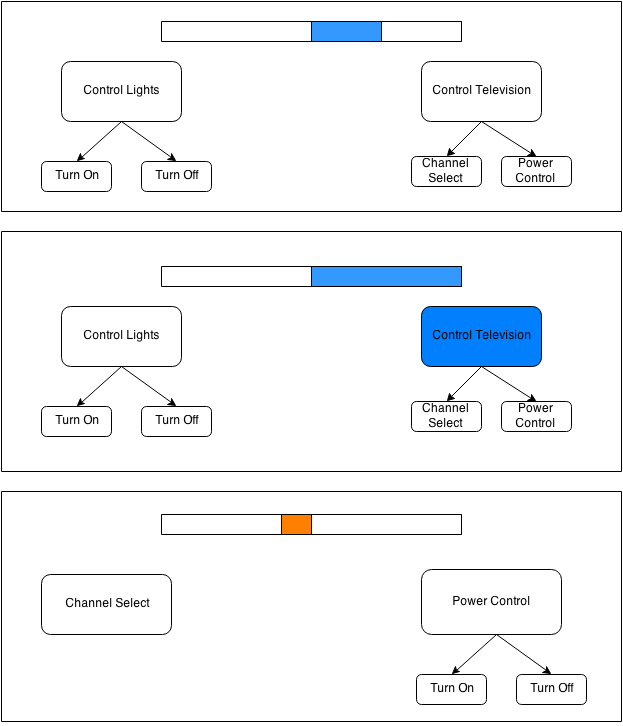
\includegraphics[width=\textwidth]{mockup_v1.png}
% TODO Kevin: fix this stupid picture. And caption
\caption{As the user concentrates, the bar fills up. When it reaches the end, the next binary choice will take its place}
\label{fig:mockup}
\end{figure}

\subsection{Functions}

%Template
%\textbf{SR2XX - NAME}
%\begin{description}
%    \item[Input:]
%    \item[Action:]
%    \item[Output:]
%    \item[Notes:] 
%    \item[Priority:]
%\end{description}

\textbf{SR205 - Calibrate}
\begin{description}
    \item[Input:] EEG data, supporting data from Caretaker
    \item[Action:] Derive calibration parameters for the Patient
    \item[Output:] Calibration parameters (internal; to be saved)
    \item[Notes:] The parameters (including the input thoughts requested from
        the user) should be chosen to give a reliable signal. Recalibration
        should be possible, as Patients' thought patterns may change over
        time.
    \item[Priority:] Must Have
\end{description}

\hfill \\

\textbf{SR210 - Activate menu via EEG}
\begin{description}
    \item[Input:] EEG data
    \item[Action:] Detect activation signal
    \item[Output:] Display menu
    \item[Notes:] Necessary for fully-paralyzed patients; others may have some
        other method of activation. Depends on calibration data.
    \item[Priority:] Must Have
\end{description}

\hfill \\

\textbf{SR215 - Perform Home Automation Action}
\begin{description}
    \item[Input:] EEG data
    \item[Action:] Interpret signal as menu selections
    \item[Output:] Signal to HAS corresponding to user request
    \item[Notes:] Depends on calibration data
    \item[Priority:] Must Have
\end{description}
\addtocontents{toc}{\protect\setcounter{tocdepth}{2}}
\subsection{Performance Requirements}

\textbf{SR305} The system must use less than 512 MB of RAM at all times while running.

\textbf{SR310} The system must use less than 5 GB of persistent storage space when installed.

\textbf{SR315} The system must run smoothly on a 3.2 GHz Intel i3 processor.

\textbf{SR320} The system will support one and only one terminal.

\textbf{SR325} The system will support one and only one user at a time.

\textbf{SR330} 90\% of time, menu selection must take less than 5 seconds.

\textbf{SR335} A trained user must be able to select 10 options within 2
minutes.

\subsection{Logical Database Requirements}

\textbf{SR405} The system must store calibration data for at least one user.

\subsection{Design Constraints}

% Removed the paragraph that was here because this section is for specific
% requirements. If we want to say something here, it should be a concise,
% numbered description of a requirement for the system.

\subsubsection{Standards Compliance}

The system does not need to comply with any external standards.

\subsection{Software System Attributes}

\subsubsection{Reliability} 

\textbf{SR612} The system must fail to detect a selection no more than 10\% of
the time.

\textbf{SR615} The system must incorrectly register user input no more than
once every 30 minutes.

\subsubsection{Availability}

\textbf{SR622} The system must be able to run for 24 hours without restarting
99\% of the time.

\subsubsection{Security}

\textbf{SR632} The system must have no network communication.

\textbf{SR635} The system must not log client interactions other than storing
calibration data.

\subsubsection{Maintainability}

\textbf{SR642} The menu selections must be defined by a configuration file.

\textbf{SR645} The set of available supported Insteon devices must be editable
through a configuration file.

\textbf{SR650} The system must provide a code-level interface for additional
types of Insteon devices to be added.

\subsubsection{Portability}

\textbf{SR652} The system must run on all Windows 7 and Windows 8 machines
meeting the minimum requirements.

\addtocontents{toc}{\protect\setcounter{tocdepth}{3}}
%TODO: fix bottom

\newpage
\section*{\centering Table of Contributions}
\begin{tabular}{| l | l | l | l |}
    \hline
     & Section & Writing & Editing \\
    \hline \hline
		1 & 2.2, 2.6, 3.3, 3.4, 3.6 & Kyle Patron & Michael Conway\\ \hline
		2 & 1, 2.1, 3.1 & Joe Muoio & Michael Conway\\ \hline
		3 & 2.4, 2.5 & Sam Bever & Michael Conway\\ \hline
		4 & 3.2 & Michael Conway & Kevin Zakszewski \\ \hline
		5 & 1, 2.3 & Kevin Zakszewski & Michael Conway \\ \hline
\end{tabular}
\newpage
\noindent I certify that:
\begin{itemize}
\item This paper/project/exam is entirely my own work.
\item I have not quoted the words of any other person from a printed source or a website without indicating what has been quoted and providing an appropriate citation.
\item I have not submitted this paper / project to satisfy the requirements of any other course.
\end{itemize}

\vspace{1cm}
\noindent\makebox[\textwidth][l]{
Signature:
\makebox[5cm][l] {\underline{Samuel Bever}} 
\ \ Date:
\makebox[4cm][l] {\underline{\required\today}} 
}


\vspace{0.5cm}
\noindent\makebox[\textwidth][l]{
Signature:
\makebox[5cm][l] {\underline{Michael Conway}} 
\ \ Date:
\makebox[4cm][l] {\underline{\required\today}} 
}

\vspace{0.5cm}
\noindent\makebox[\textwidth][l]{
Signature:
\makebox[5cm][l] {\underline{Joe Muoio}} 
\ \ Date:
\makebox[4cm][l] {\underline{\required\today}} 
}

\vspace{0.5cm}
\noindent\makebox[\textwidth][l]{
Signature:
\makebox[5cm][l] {\underline{Kyle Patron}} 
\ \ Date:
\makebox[4cm][l] {\underline{\required\today}} 
}

\vspace{0.5cm}
\noindent\makebox[\textwidth][l]{
Signature:
\makebox[5cm][l] {\underline{Kevin Zakszewski}} 
\ \ Date:
\makebox[4cm][l] {\underline{\required\today}} 
}

\vspace{\fill}
\subsection*{Grading}
The grade is given on the basis of quality, clarity, presentation, completeness, and writing of each section in the report. This is the grade of the group. Individual grades will be assigned at the end of the term when peer reviews are collected.
\end{document}
